\documentclass[12pt]{article}

\usepackage[utf8]{inputenc}
\usepackage[T1]{fontenc}
\usepackage[brazil]{babel}
\usepackage{sbc-template}
\usepackage{graphicx}
\usepackage[hyphens]{url}
\usepackage[hidelinks]{hyperref}

% O template embute um ponto no contador de seção, e o \ref herda ("Seção 2."). Aqui o ponto fica só no título.
\makeatletter
\renewcommand{\thesection}{\arabic{section}}
\renewcommand{\thesubsection}{\thesection.\arabic{subsection}}
\renewcommand{\@seccntformat}[1]{\csname the#1\endcsname.\quad}
\makeatother

\sloppy

\title{Aplicação de Práticas de Engenharia de Software Seguro em um Sistema de Transcrição de Mídias para um Ministério Público Estadual}

\author{Alexandre Alves\inst{1}, Bruno Monteiro\inst{1}, Carlos Martins\inst{1}, Gabriel Rocha\inst{1}}

\address{Programa de Pós-Graduação em Ciência da Computação (PPGCO)\\
  Universidade Federal de Uberlândia (UFU) -- Uberlândia -- MG -- Brasil
  \email{\parbox{.95\textwidth}{\centering\ttfamily\small
    alexandre.henrick@ufu.br, bruno.monteiro@ufu.br,\\
    carlos.martins1@ufu.br, gabriel.gomes1@ufu.br}}
}

\begin{document}

    \maketitle

    \begin{abstract}
        A fazer
    \end{abstract}

    \begin{resumo}
        A fazer
    \end{resumo}

    \section{Introdução}
    \label{sec:intro}

    Os Ministérios Públicos estaduais lidam com um volume crescente de mídias anexadas a processos, como gravações de depoimentos, oitivas e inquéritos, muitas delas com horas de duração. Para usar esse material, o promotor precisa ouvi-lo por inteiro ou depender de uma transcrição manual que é lenta e cara. Modelos de reconhecimento de fala treinados em larga escala tornaram viável a transcrição automática de áudios longos e em vários idiomas, incluindo o português \cite{radford:23}. Com isso, surgem serviços que, além de transcrever, permitem consultar o texto transcrito com apoio de inteligência artificial (IA).

    Um serviço desse tipo, porém, concentra informação sensível. As mídias e as transcrições trazem dados de processos sigilosos e dados pessoais de vítimas, testemunhas e investigados, e o próprio uso do serviço revela em quais processos cada promotor atua. O serviço depende ainda de sistemas que não controla: o Sistema Processos do Estado, o provedor de identidade institucional e uma IA externa acessada por API. Além disso, é compartilhado por todos os promotores do Estado, que não devem ter acesso aos dados uns dos outros. Uma falha de autorização ou de integração expõe processos sigilosos e dados pessoais.

    Em sistemas com esse perfil, a segurança precisa ser tratada desde a concepção e ao longo de todo o ciclo de desenvolvimento,
    e não acrescentada depois que o software está pronto \cite{mcgraw:06}. É essa a proposta de processos como o SDL (\textit{Security Development Lifecycle}) \cite{howard:06} e o SSDF (\textit{Secure Software Development Framework}) \cite{nist:ssdf}, que encadeiam a análise de ameaças, os requisitos de segurança, o projeto, a codificação e a verificação.

    Este artigo relata a aplicação dessas práticas a um serviço de transcrição de mídias por IA para um Ministério Público (MP) estadual, desenvolvido como trabalho da disciplina de Engenharia de Software Seguro. O serviço é um caso fictício, mas modelado com componentes e restrições próximos dos de um sistema real. Sobre ele foram aplicadas, em sequência, a modelagem de ameaças com STRIDE e casos de abuso \cite{kohnfelder:99,shostack:14}, a priorização e o tratamento dos riscos segundo o NIST CSF (\textit{Cybersecurity Framework}) 2.0 \cite{nist:csf2}, a arquitetura segura, a implementação de duas práticas de código seguro com os testes definidos antes do código e a verificação dinâmica do protótipo com o ZAP (\textit{Zed Attack Proxy}). A principal contribuição é a rastreabilidade entre essas etapas. Cada prática implementada remonta a uma ameaça, a um risco, a um requisito de segurança e a uma vulnerabilidade catalogada, e termina em testes automatizados e em evidências de verificação.

    O restante do artigo está organizado da seguinte forma. A Subseção~\ref{sec:servico} apresenta o serviço analisado. A Seção~\ref{sec:stride} descreve a modelagem de ameaças; a Seção~\ref{sec:riscos}, a priorização e o tratamento dos riscos; a Seção~\ref{sec:arquitetura-segura}, os requisitos e as decisões de arquitetura segura; a Seção~\ref{sec:codigo-seguro}, a implementação das práticas de código seguro; e a Seção~\ref{sec:verificacao}, a verificação de vulnerabilidades. As Seções~\ref{sec:monitoramento} e \ref{sec:devsecops} abordam, respectivamente, o monitoramento e a detecção de intrusões e o \textit{pipeline} DevSecOps, e a Seção~\ref{sec:conclusao} apresenta as conclusões.

    \subsection{O serviço analisado}
    \label{sec:servico}

    O serviço é usado pelos promotores do Estado para obter a versão textual de mídias de longa duração vinculadas a processos. O promotor consulta um processo, escolhe uma das mídias disponíveis e solicita a transcrição. O Backend copia a mídia para o Storage e publica um pedido em uma fila.
    O Módulo IA, um serviço em Python que consome essa fila, envia a mídia a uma IA externa, grava a transcrição no Storage e informa o Backend da mudança de status. Com a transcrição finalizada, o promotor pode abri-la, baixá-la em formato .docx, excluí-la ou usá-la como contexto em um chat com a IA. A Figura~\ref{fig:hld} mostra os componentes e as interações entre eles.

    \begin{figure}[htbp]
        \centering
        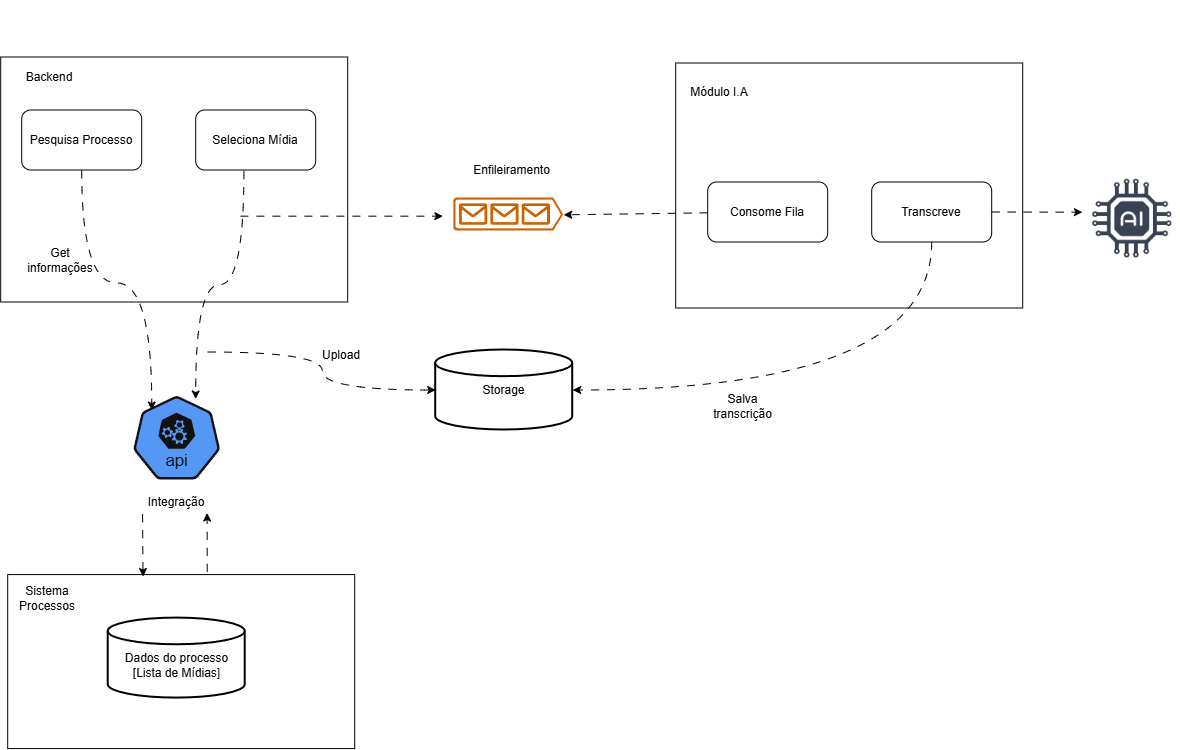
\includegraphics[width=.85\textwidth]{hldesign.png}
        \caption{Arquitetura em alto nível do serviço de transcrição.}
        \label{fig:hld}
    \end{figure}

    Algumas fronteiras de escopo restringem o que pode ser modelado. As mídias são incluídas nos processos por atores externos, como polícia e cartórios, dentro do Sistema Processos. O serviço apenas lê processos e mídias pela API desse sistema e nunca escreve nele, e o promotor não faz \textit{upload} de arquivos. O serviço confia na decisão de autorização por processo devolvida por essa API, mas não confia no conteúdo do arquivo recebido, cujo formato, tamanho e ausência de conteúdo malicioso são validados antes da cópia para o Storage. O cadastro e a desativação de promotores ficam no provedor de identidade institucional: o Backend apenas valida o token de identidade emitido por ele e cria a sessão local. No chat, o Backend chama a IA diretamente, e o histórico da conversa fica em memória e é descartado quando o chat é encerrado. A Tabela~\ref{tab:ativos} lista os ativos que orientaram a modelagem de ameaças. Os requisitos funcionais RQF1 a RQF11, citados pelos identificadores nas seções seguintes, cobrem o acesso com credenciais institucionais (RQF1), a pesquisa de mídias e a solicitação da transcrição (RQF2 e RQF3), o acompanhamento do status (RQF4), a listagem, a abertura, o \textit{download} e a exclusão de transcrições (RQF5, RQF6, RQF8 e RQF9), o chat com a IA sobre uma transcrição (RQF7 e RQF10) e o encerramento da sessão (RQF11).

    \begin{table}[htbp]
        \centering
        \caption{Ativos do serviço.}
        \label{tab:ativos}
        \footnotesize
        \begin{tabular}{|c|p{5.2cm}|p{7.4cm}|}
            \hline
            \textbf{ID} & \textbf{Ativo} & \textbf{Descrição} \\
            \hline
            A1 & Credenciais & Credenciais de acesso dos promotores \\
            \hline
            A2 & Dados de processos & Dados de processos de natureza jurídica de todo o Estado \\
            \hline
            A3 & Mídias & Áudios e vídeos vinculados aos processos de A2 \\
            \hline
            A4 & Informações de cunho profissional & Em quais processos cada promotor está atuando \\
            \hline
            A5 & Informações pessoais & Dados pessoais contidos nos processos de A2 \\
            \hline
            A6 & Interações com a IA & Perguntas e respostas trocadas entre o promotor e a IA \\
            \hline
        \end{tabular}
    \end{table}

    \section{Modelagem de Ameaças com STRIDE}
    \label{sec:stride}

    A modelagem de ameaças identifica, ainda na fase de projeto, o que pode dar errado em um sistema, antes que essas falhas se tornem vulnerabilidades no código \cite{shostack:14,xiong:19}.
    A técnica adotada foi o STRIDE, proposto na Microsoft \cite{kohnfelder:99} e incorporado ao SDL \cite{howard:06}.
    O nome reúne seis categorias de ameaça, cada uma associada a uma propriedade de segurança violada: falsificação de identidade (\textit{Spoofing}) viola a autenticidade; adulteração (\textit{Tampering}), a integridade; repúdio (\textit{Repudiation}), o não repúdio; divulgação de informação (\textit{Information Disclosure}), a confidencialidade; negação de serviço (\textit{Denial of Service}), a disponibilidade; e elevação de privilégio (\textit{Elevation of Privilege}), a autorização \cite{shostack:14}.

    A análise partiu dos componentes da Figura~\ref{fig:hld} e dos diagramas de sequência elaborados para cada requisito funcional. Esses diagramas mostram as mensagens trocadas entre o promotor, o Backend, o provedor de identidade, o Sistema Processos, o Storage, a fila, o Módulo IA e a IA externa. Para cada interação, a análise verificou quais categorias do STRIDE se aplicavam, considerando as premissas da Seção~\ref{sec:servico}. Cada ameaça foi registrada com um identificador, a categoria, os ativos afetados, os requisitos envolvidos e uma descrição do cenário. Em seguida, as ameaças mais relevantes foram detalhadas como casos de abuso, narrativas curtas escritas do ponto de vista de quem ataca o sistema \cite{mcdermott:99,sindre:05}.

    \subsection{Ameaças identificadas}

    Foram catalogadas 16 ameaças, resumidas na Tabela~\ref{tab:stride}; a elevação de privilégio concentra seis delas, e nenhuma se enquadrou em repúdio.

    \begin{table}[htbp]
        \centering
        \caption{Ameaças identificadas com o STRIDE. Categorias: S, falsificação de identidade; T, adulteração; I, divulgação de informação; D, negação de serviço; E, elevação de privilégio.}
        \label{tab:stride}
        \footnotesize
        \begin{tabular}{|c|p{8.4cm}|c|p{2.8cm}|}
            \hline
            \textbf{ID} & \textbf{Ameaça} & \textbf{Cat.} & \textbf{Ativos} \\
            \hline
            AME1 & Acesso a transcrição de outro promotor & E & A2, A3, A4, A5 \\
            \hline
            AME2 & Backend como procurador confuso na consulta ao Sistema Processos & E & A2, A3, A4 \\
            \hline
            AME3 & Usuário do MP que não é promotor entra como promotor & E & A1 \\
            \hline
            AME4 & Atualização de status sem autenticação de serviço & E & A2, A3 \\
            \hline
            AME5 & Mensagem forjada na fila & E & A2, A3, A5 \\
            \hline
            AME6 & Mídia maliciosa executa código no Módulo IA & E & A2, A3, A5 \\
            \hline
            AME7 & Transcrição baixada usada fora do ambiente do MP & I & A2, A4 \\
            \hline
            AME8 & Acesso a partir de ambientes externos ao MP & I & A3 \\
            \hline
            AME9 & Volume alto de pedidos de transcrição na fila & D & A2 a A6 \\
            \hline
            AME10 & Falhas provocadas para forçar novas tentativas na IA & D & A3, A6 \\
            \hline
            AME11 & Esgotamento do Storage & D & A3 \\
            \hline
            AME12 & Sobrecarga de perguntas no chat com a IA & D & A6 \\
            \hline
            AME13 & Falsificação de identidade de um promotor & S & A1 \\
            \hline
            AME14 & Adulteração da transcrição ou de seus metadados & T & A2, A4 \\
            \hline
            AME15 & Adulteração da mídia antes da transcrição & T & A3, A5 \\
            \hline
            AME16 & Adulteração de mensagens da fila & T & A2, A3, A5 \\
            \hline
        \end{tabular}
    \end{table}

    A predominância da elevação de privilégio reflete o desenho do serviço, compartilhado por promotores que não devem ver os dados uns dos outros: boa parte das ameaças descreve um usuário ou componente legítimo que alcança dados além do que deveria. A AME1, narrada no caso de abuso CAE1, é o caso mais direto: um promotor autenticado troca o identificador da transcrição na requisição e, se o Backend não conferir a quem ela pertence, lê ou exclui a transcrição de um colega e descobre em quais processos ele atua. Essa falha corresponde à quebra de autorização em nível de objeto, primeira posição do OWASP API Security Top 10 \cite{owasp:api10}. A AME2 é um exemplo do problema do procurador confuso \cite{hardy:88}.
    A credencial do Backend na API do Sistema Processos alcança todos os processos do Estado, e a autorização por processo depende da identidade do promotor que o Backend repassa. Se essa identidade vier de um campo da requisição, e não da sessão, um promotor consulta processos que não são seus com a autoridade do Backend. A AME3 parte do fato de o provedor de identidade atender todo o Ministério Público: um token legítimo, emitido para outro sistema ou para um servidor que não é promotor, abre uma sessão se o Backend não conferir a audiência do token e o papel do usuário.

    Outro grupo de ameaças explora a confiança entre componentes internos. Na AME4, qualquer máquina que alcance o \textit{endpoint} de atualização de status marca transcrições como finalizadas e aponta o registro para outro objeto do Storage. Na AME5, quem consegue publicar na fila envia pedidos com caminhos arbitrários, e o Módulo IA, que tem acesso a todo o Storage, executa-os. Nesse cenário, o \textit{hash} da mídia incluído na mensagem não protege, porque quem forja a mensagem calcula o \textit{hash} do arquivo para o qual ela aponta. A AME6 dispensa até mesmo uma conta no sistema: uma parte do processo junta a ele uma mídia preparada para explorar o decodificador de áudio ou vídeo, e o código malicioso é executado com a credencial do Módulo IA quando um promotor, de boa-fé, pede a transcrição.

    As ameaças de negação de serviço, AME9 a AME12, tratam do esgotamento de recursos compartilhados: a fila, a cota da IA externa, o espaço do Storage e a memória que guarda o histórico dos chats. As de divulgação de informação, AME7 e AME8, envolvem o uso da transcrição baixada em serviços de terceiros e o acesso a partir de máquinas fora do ambiente do MP. Esses dois cenários dependem em parte do comportamento do usuário, e não só de controles técnicos. As ameaças de adulteração, AME14 a AME16, atingem a mídia, a mensagem na fila e a transcrição já gerada. A de falsificação de identidade, AME13, cobre o uso de credenciais ou tokens obtidos de um promotor.


    \section{Priorização e Tratamento de Riscos}
    \label{sec:riscos}

    Cada uma das 16 ameaças da Seção~\ref{sec:stride} deu origem a um risco, numerado na mesma ordem (RI01 a RI16) e avaliado por probabilidade (P) e impacto (I), ambos de 1 a 4. A pontuação $R = P \times I$ classifica o risco como baixo (1 a 4), médio (5 a 8), alto (9 a 12) ou muito alto (13 a 16). A avaliação inicial resultou em dois riscos muito altos, cinco altos, seis médios e três baixos (Tabela~\ref{tab:riscos}).

    Os dois riscos de nota 16 são RI01, em que um promotor acessa transcrições de outro, e RI07, em que uma transcrição exibida ou baixada é levada a serviços externos, fora do controle técnico do sistema. Os cinco riscos altos, RI02, RI03, RI04, RI08 e RI13, envolvem autorização, autenticação e confiança entre componentes.

    \subsection{Estratégias e plano de tratamento}

    O tratamento seguiu o NIST CSF 2.0, cujas seis funções organizam as atividades de segurança: Govern (políticas e responsabilidades), Identify (avaliação dos riscos e registro das decisões), Protect (salvaguardas preventivas), Detect (monitoramento e análise de eventos), Respond (mitigação de incidentes) e Recover (restauração após incidentes). O plano usa as categorias GV.PO, ID.RA, PR.AA, PR.DS, PR.PS, PR.IR, DE.CM, DE.AE e RS.MI; Recover não recebeu ação nova, porque a restauração usa o backup diário previsto no requisito RQNF5.7.

    Para cada risco foi escolhida uma de três estratégias: reduzir, com controles que diminuem a probabilidade ou o impacto; aceitar, por decisão registrada do responsável e com monitoramento; ou evitar, eliminando a condição que permite o risco, opção que nenhum risco exigiu. A Tabela~\ref{tab:riscos} resume, para cada risco, o nível inicial, a estratégia, o controle principal, as funções do CSF e o nível residual esperado após os controles, estimado com a mesma escala. Os controles preventivos reduzem a probabilidade; os que limitam as consequências reduzem o impacto.

    \begin{table}[htbp]
        \centering
        \caption{Riscos avaliados, com o nível inicial seguido da pontuação, a estratégia, o controle principal, as funções do NIST CSF 2.0 e o nível residual esperado. Cada risco RI\textit{n} corresponde à ameaça AME\textit{n}.}
        \label{tab:riscos}
        \footnotesize
        \setlength{\tabcolsep}{4pt}
        \renewcommand{\arraystretch}{0.92}
        \begin{tabular}{|c|p{1.5cm}|p{1.5cm}|p{5.7cm}|p{1.9cm}|p{1.5cm}|}
            \hline
            \textbf{Risco} & \textbf{Inicial} & \textbf{Estra\-tégia} & \textbf{Controle principal} & \textbf{Funções CSF} & \textbf{Residual} \\
            \hline
            RI01 & Muito alto (16) & Reduzir & Conferência de propriedade em toda rota com identificador, identificadores UUID versão 4 e alerta em acesso negado. & PR.AA, DE.AE & Baixo (4) \\
            \hline
            RI02 & Alto (12) & Reduzir & Identidade repassada ao Sistema Processos tirada só da sessão; alerta se a requisição trouxer identidade. & PR.AA, DE.AE & Baixo (4) \\
            \hline
            RI03 & Alto (9) & Reduzir & Só token do fluxo institucional, com audiência do serviço e papel de promotor. & PR.AA & Baixo (3) \\
            \hline
            RI04 & Alto (12) & Reduzir & TLS mútuo no \textit{endpoint} de status com certificado exclusivo do Módulo IA; sem caminhos na mensagem nem alteração após finalizada. & PR.AA, DE.AE & Baixo (4) \\
            \hline
            RI05 & Médio (8) & Reduzir & Credenciais da fila separadas (Backend publica, Módulo IA consome) e mensagens assinadas com chave em cofre. & PR.AA, PR.DS, DE.AE & Baixo (4) \\
            \hline
            RI06 & Baixo (4) & Reduzir & Decodificação em contêiner descartável, sem rede nem credenciais, com limites de tempo e memória; decodificador atualizado em até 7 dias. & ID.RA, PR.PS, PR.IR, DE.AE & Baixo (2) \\
            \hline
            RI07 & Muito alto (16) & Aceitar & Decisão formal da gestão do MP, regra contra envio a serviços externos e registro de cada \textit{download}. & GV.PO, ID.RA, DE.CM & Muito alto (16) \\
            \hline
            RI08 & Alto (9) & Reduzir & Sessão expira após 15 minutos sem interação ou 8 horas; \textit{download} e exclusão pedem nova autenticação. & PR.AA, DE.CM & Médio (6) \\
            \hline
            RI09 & Médio (6) & Reduzir & Até 10 solicitações simultâneas por promotor, 3 de mídias grandes; espera acima de 30 minutos gera alerta. & PR.IR, DE.CM & Baixo (4) \\
            \hline
            RI10 & Baixo (4) & Aceitar & Sem controle novo; a operação acompanha as falhas da IA por promotor. & ID.RA, DE.CM & Baixo (4) \\
            \hline
            RI11 & Médio (6) & Reduzir & Mídia removida ao finalizar; mídia com falha retida 7 dias; ocupação acima de 80\% gera alerta. & PR.IR, DE.CM & Baixo (3) \\
            \hline
            RI12 & Médio (6) & Reduzir & Até 2 chats por promotor, 3 perguntas por minuto e 20 interações guardadas por conversa. & PR.IR & Baixo (2) \\
            \hline
            RI13 & Alto (12) & Reduzir & Segundo fator obrigatório, conferido pelo \textit{claim} \texttt{amr}; alerta em acesso de origem nunca usada, com confirmação e revogação de sessões. & PR.AA, DE.AE, RS.MI & Médio (8) \\
            \hline
            RI14 & Baixo (4) & Aceitar & Sem controle novo; valem o bloqueio de sobrescrita (RQNF6.2) e os eventos de auditoria (RQNF6.3). & ID.RA, DE.CM & Baixo (4) \\
            \hline
            RI15 & Médio (8) & Reduzir & \textit{Hash} da mídia na mensagem assinada e gravação no Storage só pelo Backend; divergência gera falha e alerta. & PR.DS, PR.AA, DE.AE & Baixo (4) \\
            \hline
            RI16 & Médio (8) & Reduzir & Os mesmos controles de RI05. & PR.AA, PR.DS, DE.AE & Baixo (4) \\
            \hline
        \end{tabular}
    \end{table}

    Os responsáveis se distribuem entre desenvolvimento do Backend e do Módulo IA, infraestrutura, operação do serviço e gestão do MP. Quando o controle depende de sistema externo, como o provedor de identidade em RI03 e RI13, a dependência deverá ser confirmada pelo respectivo responsável.

    \subsection{Aceite, risco residual e ordem de implementação}

    O RI07 permanece muito alto porque a única forma de reduzir sua probabilidade seria retirar a visualização e o \textit{download} das transcrições, que são a finalidade do serviço. Seu aceite exige decisão formal da gestão do MP, dona dos riscos, e reavaliação a cada 12 meses. Todo risco com residual médio ou superior (RI07, RI08 e RI13) e todo risco aceito (também RI10 e RI14) exige essa decisão registrada, conforme a subcategoria ID.RA-06, além da comprovação dos controles. Os riscos com residual baixo são aceitos mediante as evidências previstas no plano: testes automatizados, configurações dos componentes, registros de auditoria e confirmação das dependências externas. Se uma evidência não for produzida, um teste falhar ou uma dependência não for confirmada, o risco volta ao nível inicial e é reavaliado.

    A ordem de implementação segue a criticidade e a dependência entre controles: primeiro autenticação e autorização (RI01, RI02, RI03 e RI13), que estabelecem a identidade usada pelos demais; depois a comunicação entre serviços e o processamento de mídias (RI04 e RI06); em seguida a integridade (RI05, RI15 e RI16); o aceite formal e o registro de \textit{downloads} de RI07; e, por último, os limites de uso e a remoção de mídias (RI08, RI09, RI11 e RI12). RI10 e RI14, aceitos sem controle novo, ficam fora da sequência. Os riscos RI01, RI13 e RI04 orientaram os requisitos e as decisões de arquitetura da Seção~\ref{sec:arquitetura-segura}.

    \section{Arquitetura Segura}
    \label{sec:arquitetura-segura}

    Três riscos da Seção~\ref{sec:riscos} orientaram a arquitetura, um em cada ponto de confiança do serviço: RI01, na autorização do Backend; RI13, na autenticação do promotor; e RI04, na autenticação entre serviços. RI07 ficou de fora por ser aceito, e RI02 e RI03 são cobertos pelas mesmas decisões de RI01 e RI13, porque a identidade repassada ao Sistema Processos passa a vir só da sessão e o token passa a ser validado por audiência e papel. Cada risco gerou um requisito de segurança derivado do controle do plano de tratamento, com um critério de verificação, e recebeu uma vulnerabilidade de catálogo que o descreve (Tabela~\ref{tab:requisitos}).

    \begin{table}[htbp]
        \centering
        \caption{Requisitos de segurança, com o risco de origem, o critério de verificação e a vulnerabilidade de catálogo que cada um trata.}
        \label{tab:requisitos}
        \footnotesize
        \setlength{\tabcolsep}{4pt}
        \begin{tabular}{|p{1.3cm}|p{4.3cm}|p{4.2cm}|p{3.7cm}|}
            \hline
            \textbf{ID} & \textbf{Requisito} & \textbf{Critério de verificação} & \textbf{Vulnerabilidade} \\
            \hline
            RS01 (RI01) & O Backend confere, em toda rota que recebe identificador de transcrição ou chat (RQF4, RQF6 a RQF10), que o recurso pertence ao promotor da sessão, e gera esses identificadores como UUID versão 4. & Com sessões de dois promotores, A e B, cada rota chamada por A com identificador de B responde acesso negado, sem dado, sem alteração e com alerta; identificadores criados em sequência não têm relação entre si. & V01: autorização contornada por chave controlada pelo usuário. CWE-639 e CWE-340; OWASP Top 10 2021 A01; API Security Top 10 2023 API1; ASVS 5.0 8.2.2 e 8.3.1. \\
            \hline
            RS02 (RI13) & O Backend cria a sessão (RQF1) somente a partir de token de identidade que comprove segundo fator, pelo \textit{claim} \texttt{amr} contendo \texttt{mfa} \cite{rfc8176}, e recusa qualquer outro token, mesmo com assinatura, emissor, audiência e prazo válidos. & Token assinado pelo provedor, válido, mas sem indicação de segundo fator, não cria sessão e não abre nenhuma rota de dados; o mesmo token com \texttt{mfa} cria a sessão. & V02: autenticação de fator único. CWE-308; OWASP Top 10 2021 A07; ASVS 5.0 6.3.3 e 10.3.4. \\
            \hline
            RS03 (RI04) & O \textit{endpoint} de status (RQF4) aceita somente chamadas com TLS mútuo e o certificado de cliente exclusivo do Módulo IA, recebe apenas identificador, status e \textit{hash} do texto ou motivo da falha, deriva o caminho no Storage do identificador e não altera transcrição finalizada. & Chamadas sem certificado, com certificado de outro serviço ou revogado são recusadas antes de ler o registro; chamadas com campo de caminho ou que mudam transcrição finalizada são recusadas sem alterar nada; cada recusa gera alerta. & V03: falta de autenticação em função crítica. CWE-306 e CWE-73; OWASP Top 10 2021 A07; API Security Top 10 2023 API2; ASVS 5.0 12.1.3 e 12.3.5. \\
            \hline
        \end{tabular}
    \end{table}

    A Figura~\ref{fig:arquitetura} posiciona os controles na arquitetura. A autenticação (AUTN) valida o token e cria a sessão local, e é onde RS02 atua. A autorização (AUTZ) confere a sessão em toda requisição, decide o acesso a transcrições e processos e publica os pedidos na fila, e é onde RS01 atua. O \textit{endpoint} de status (ST) recebe do Módulo IA a atualização de cada transcrição, e é onde RS03 atua. Os três pontos, mais o Módulo IA, enviam recusas, acessos negados, \textit{downloads} e falhas de \textit{hash} para os registros e alertas, que a Seção~\ref{sec:monitoramento} consome.

    \begin{figure}[htbp]
        \centering
        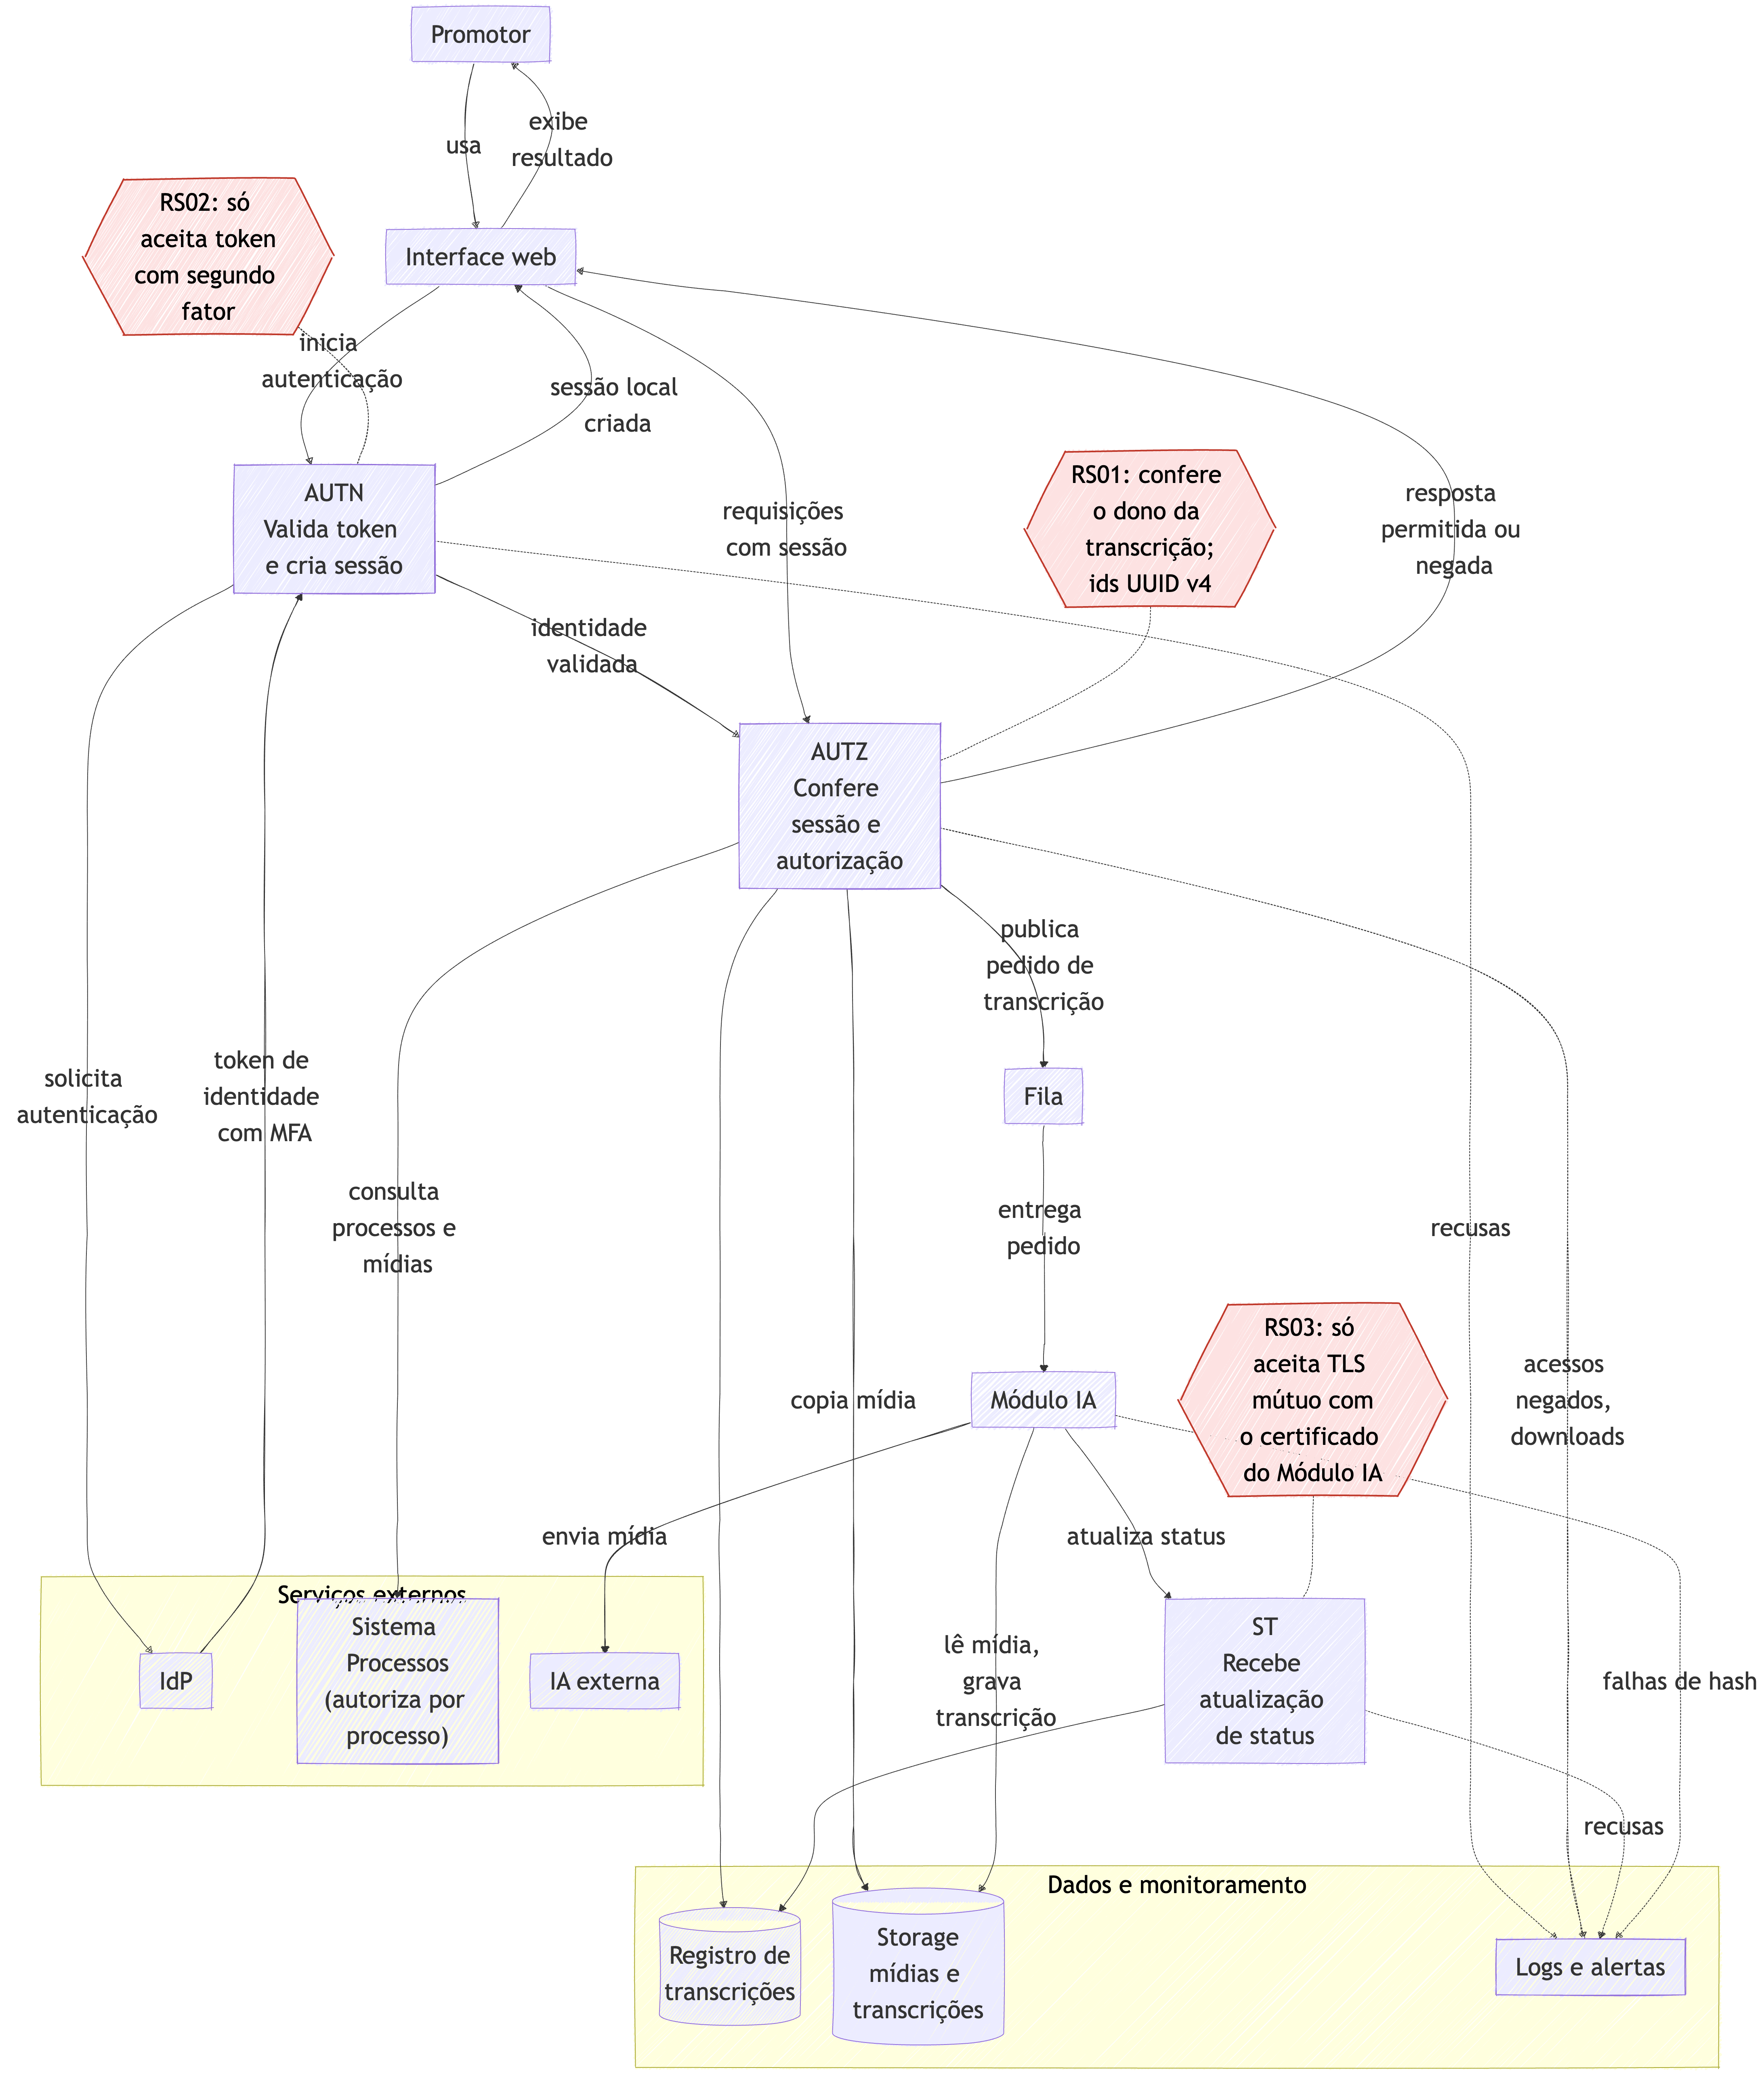
\includegraphics[width=.9\textwidth]{arquitetura-segura.png}
        \caption{Arquitetura segura do serviço, com os pontos de autenticação (AUTN), autorização (AUTZ) e atualização de status (ST) e a posição dos requisitos RS01 a RS03.}
        \label{fig:arquitetura}
    \end{figure}

    Cada requisito virou uma decisão de arquitetura com critério de aceitação. A DA01 implementa a autorização no Backend: a identidade do promotor autenticado valida a propriedade de cada transcrição ou chat antes de qualquer consulta, \textit{download}, exclusão ou outra operação, e os identificadores são UUID (\textit{Universally Unique Identifier}) versão 4; o critério é que, com dois promotores, nenhum acesse, altere, baixe ou exclua recurso do outro. A DA02 integra o Backend ao provedor de identidade institucional com autenticação multifator (MFA) obrigatória: o Backend valida o token e confirma a indicação de segundo fator antes de criar a sessão; o critério é que um token válido sem MFA seja recusado e o mesmo token com MFA crie a sessão. A DA03 implementa a autenticação entre serviços com TLS mútuo e certificado exclusivo do Módulo IA: o Backend valida o certificado antes de aceitar a atualização de status e controla os campos que podem mudar; o critério é que chamadas sem certificado, com certificado inválido ou de outro serviço sejam recusadas, e uma chamada com certificado válido e campos permitidos atualize o status. As decisões DA01 e DA02 foram implementadas no protótipo da Seção~\ref{sec:codigo-seguro}; a DA03 depende do Módulo IA, que fica fora do protótipo.

    \section{Código Seguro}
    \label{sec:codigo-seguro}

    As decisões DA01 e DA02 da Seção~\ref{sec:arquitetura-segura} foram implementadas em um protótipo do serviço de transcrição, escrito em Java 21 com Spring Boot e executado por Docker Compose. A escolha considerou a criticidade dos riscos e a possibilidade de demonstrar os controles por testes automatizados.
    O protótipo cobre o necessário para exercitar as práticas: criação e encerramento de sessão (RQF1 e RQF11), listagem, abertura e exclusão de transcrições (RQF5, RQF6 e RQF9), um provedor de identidade simulado e um registro de transcrições em banco H2 em memória com dados de dois promotores.
    Os testes de segurança usam JUnit 5 com MockMvc e inicializam a aplicação inteira.
    Em cada prática a ordem de trabalho foi a mesma: a tabela de testes entrou primeiro no documento, depois a classe de teste, que falhou, e por fim a implementação, que a fez passar.

    \subsection{Prática 1: sessão criada somente com segundo fator}

    A prática atende ao requisito RS02 e trata o risco RI13 ao mitigar a vulnerabilidade V02, autenticação de fator único (CWE-308).
    A conta do promotor é institucional, e uma senha obtida por \textit{phishing} ou reutilizada fora do órgão não pode bastar para abrir sessão.
    O Backend recebe do provedor de identidade um JWT (\textit{JSON Web Token}) e o valida: algoritmo de assinatura RS256, assinatura com a chave pública do provedor, emissor, audiência, prazo e sujeito.
    Em seguida, confere o \textit{claim} \texttt{amr} \cite{rfc8176} e exige que ele contenha o valor \texttt{mfa}.
    Um token íntegro e dentro do prazo, mas emitido apenas com senha, recebe a resposta genérica de erro de autenticação; o motivo fica no \textit{log} do servidor, para não orientar quem forja tokens.

    Quando o token é aceito, o Backend não o reaproveita como credencial.
    Ele gera um token de sessão opaco, com 256 bits de um gerador criptográfico, guarda-o em memória e o devolve ao cliente.
    A partir daí, só esse token circula, no cabeçalho \texttt{Authorization}, e o encerramento da sessão o invalida.
    O provedor de identidade é simulado dentro da aplicação: gera um par de chaves RSA a cada início, mantém a chave privada só em memória e emite tokens com ou sem o segundo fator, o que permite demonstrar a recusa na interface.

    \subsection{Prática 2: autorização por propriedade do recurso}

    Esta prática cobre o requisito RS01 e trata o risco RI01 ao mitigar a vulnerabilidade V01: um promotor troca o identificador na requisição e lê ou apaga a transcrição de um colega (CWE-639), o que identificadores previsíveis facilitam (CWE-340).
    A implementação delega ao repositório a comparação com o dono da sessão, pela consulta \texttt{findByIdAndPromotorId}; assim, o registro de outro promotor nem chega a ser carregado.
    Identificador alheio e identificador inexistente produzem resposta idêntica, 403 com a mensagem \texttt{acesso negado}, para não revelar quais identificadores existem.
    Cada recusa gera um registro de auditoria com promotor, operação e identificador, sem o conteúdo da transcrição.
    Os identificadores são UUID versão 4 gerados pela entidade, sem sequência no banco.

    \subsection{Testes e resultados}

    A Tabela~\ref{tab:testes} resume os seis testes definidos antes da implementação, TS01 a TS06, escritos em nove métodos na entrega da Etapa 4: TS04 em três, TS05 em dois e os demais em um método cada.

    \begin{table}[htbp]
        \centering
        \caption{Testes de segurança das duas práticas, definidos antes da implementação: TS01 a TS03 cobrem a sessão com segundo fator, e TS04 a TS06, a autorização por propriedade do recurso.}
        \label{tab:testes}
        \footnotesize
        \begin{tabular}{|c|p{6cm}|p{5.4cm}|}
            \hline
            \textbf{Teste} & \textbf{Entrada ou ação} & \textbf{Resultado esperado} \\
            \hline
            TS01 & Token assinado pelo provedor, válido, com o \textit{claim} \texttt{amr} contendo só \texttt{pwd} & 401 sem token de sessão; nenhuma rota de dados abre \\
            \hline
            TS02 & O mesmo token com \texttt{amr} contendo \texttt{pwd} e \texttt{mfa} & 200 com token de sessão; a listagem responde 200 \\
            \hline
            TS03 & Tokens com \texttt{mfa} mas assinados por outra chave, com audiência de outro serviço ou expirados & 401 nos três \\
            \hline
            TS04 & Promotor A abre e exclui a transcrição de B, e abre um identificador inexistente & 403 nas três chamadas, sem dados, sem alteração e com registro de auditoria \\
            \hline
            TS05 & Promotor A abre e exclui a própria transcrição & 200 com o texto; 204 e o registro deixa de existir; nenhum registro de auditoria \\
            \hline
            TS06 & Duas transcrições criadas em sequência & Identificadores UUID versão 4 e diferentes entre si \\
            \hline
        \end{tabular}
    \end{table}

    Com as classes de teste no repositório e sem os \textit{controllers}, os três métodos da Prática 1 falharam por rota inexistente: TS01 e TS03 receberam 404 em vez de 401, e TS02 recebeu 404 em vez de 200.
    Na Prática 2, cinco dos seis métodos falharam pela mesma razão; TS06 já passava, porque a geração do identificador entrou com o modelo.
    Após a implementação, os nove métodos passam.
    O \textit{build} da imagem Docker executa a suíte, e um teste reprovado impede a inicialização da aplicação.

    \section{Verificação de Vulnerabilidades}
    \label{sec:verificacao}

    O protótipo foi verificado com o ZAP (\textit{Zed Attack Proxy}) 2.17.0, em um contêiner adicional do mesmo Docker Compose, que alcança a aplicação pela rede interna.
    Um \textit{script} controla o ZAP pela API e executa a rodada de verificação em três etapas.
    Primeiro, o \textit{script} repete pelo \textit{proxy} o fluxo de uso e os abusos levantados nas etapas anteriores: \textit{login} sem segundo fator, token com o conteúdo adulterado e a assinatura original, \textit{claim} \texttt{amr} forjado, assinatura inválida, rotas de dados sem sessão, promotor abrindo e excluindo transcrição de colega, identificador inexistente e identificador fora do formato.

    Depois, executa o \textit{spider}, que segue os links das páginas para completar a lista de URLs; o \textit{scan} passivo, que examina cabeçalhos e corpo de cada resposta registrada sem enviar requisição e é a origem dos alertas de cabeçalho; e o \textit{scan} ativo, que reenvia cada requisição com variações de ataque, usando a sessão de um promotor no cabeçalho \texttt{Authorization} e injetando \textit{payloads} em parâmetros de consulta, no corpo JSON e nos segmentos de caminho, onde ficam os identificadores.
    A rota \texttt{/api/sessao} ficou fora do \textit{scan} ativo, porque um \texttt{DELETE} derrubaria a sessão que o \textit{scan} usa.

    Por fim, o \textit{script} grava os relatórios em HTML e JSON, um resumo dos alertas, o registro do tráfego e os parâmetros da rodada.
    A rodada registrada no repositório teve 38 chamadas de roteiro, todas com o código de resposta esperado.
    O contexto reuniu 23 URLs e o histórico, 10.311 mensagens, 10.241 delas do \textit{scan} ativo, que durou 12 s.
    Não houve alerta de risco alto, apenas dois alertas médios, um baixo e dois informativos, como mostra a Figura~\ref{fig:zap}.
    O \textit{scan} ativo, com \textit{payloads} de injeção de SQL, XSS (\textit{Cross-Site Scripting}), travessia de diretório e injeção de comando, entre outras regras da política padrão, não gerou alerta.
    Isso é coerente com consultas JPA parametrizadas, identificadores tipados como UUID e dados inseridos no DOM apenas por \texttt{textContent}.
    A Tabela~\ref{tab:achados} resume os três achados analisados.
    Todos vêm da falta de cabeçalhos de segurança no Backend, e a correção proposta é um único filtro aplicado a toda resposta.

    \begin{figure}[htbp]
        \centering
        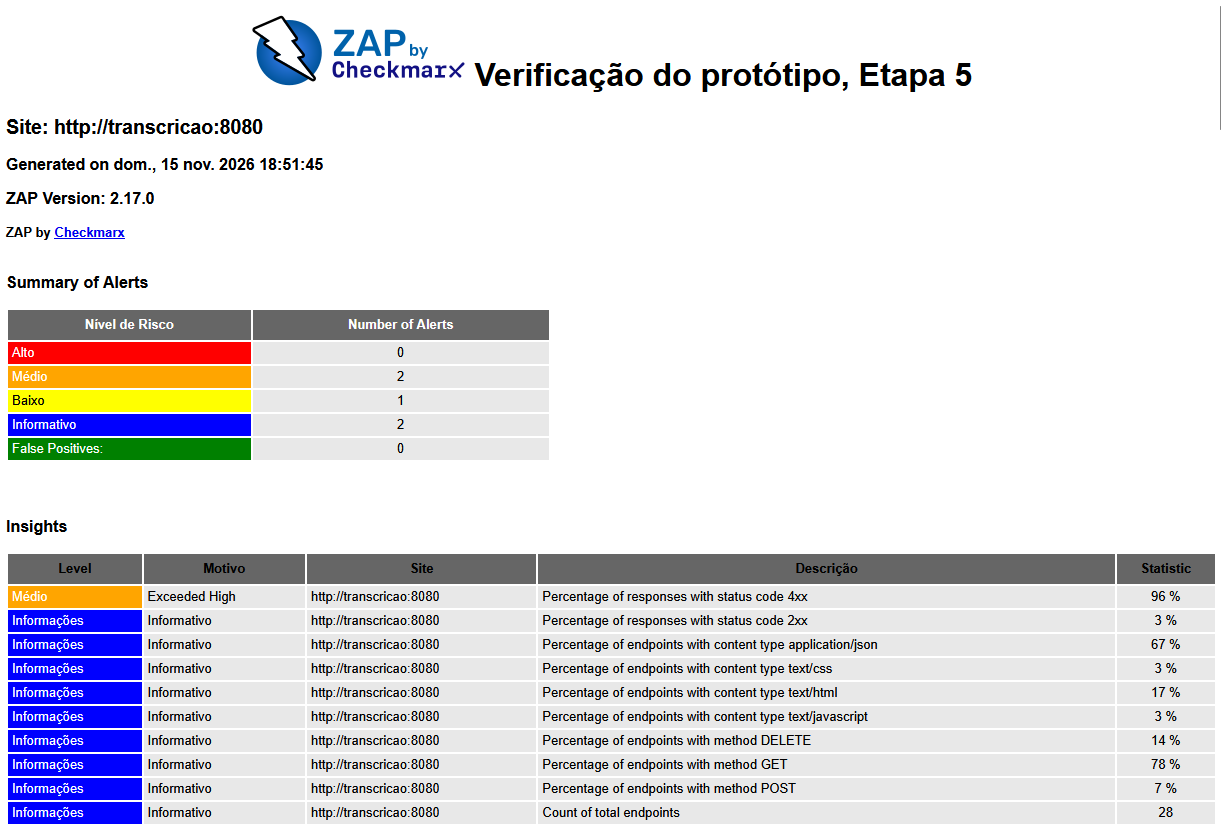
\includegraphics[width=.95\textwidth]{relatorio-zap-resumo.png}
        \caption{Resumo do relatório HTML gerado pelo ZAP ao fim da rodada: alvo, versão, contagem de alertas por nível de risco e estatísticas do histórico. Os 96\% de respostas 4xx são as requisições do \textit{scan} ativo rejeitadas pela aplicação.}
        \label{fig:zap}
    \end{figure}

    \begin{table}[htbp]
        \centering
        \caption{Achados da rodada do ZAP sobre o protótipo, com a regra que gerou cada alerta, o impacto possível, a referência de catálogo e a correção proposta.}
        \label{tab:achados}
        \footnotesize
        \begin{tabular}{|c|p{3.9cm}|p{3.3cm}|p{1.9cm}|p{3.2cm}|}
            \hline
            \textbf{ID} & \textbf{Achado} & \textbf{Possível impacto} & \textbf{Referência} & \textbf{Correção proposta} \\
            \hline
            A01 & Resposta sem \path{Content-Security-Policy} nas páginas HTML (regra 10038) & Um XSS que passe pelas defesas da interface lê o token de sessão e age como o promotor em todas as transcrições dele & CWE-693; OWASP Top 10 2021 A05 & Política \texttt{default-src 'self'}; \texttt{frame-ancestors 'none'}; \texttt{base-uri 'none'}; \texttt{form-action 'self'}, com os scripts e estilos embutidos movidos para arquivos \\
            \hline
            A02 & Resposta sem \path{X-Frame-Options} nem \path{frame-ancestors} (regra 10020) & Página embutida em quadro invisível de site hostil induz o promotor a acionar a exclusão sem perceber & CWE-1021; OWASP Top 10 2021 A05 & \path{X-Frame-Options}: \texttt{DENY} e a diretiva \texttt{frame-ancestors 'none'} \\
            \hline
            A03 & Resposta sem \path{X-Content-Type-Options} em HTML, CSS e JSON (regra 10021) & Navegador antigo reinterpreta o tipo da resposta e pode tratar o texto da transcrição como HTML & CWE-693 & \path{X-Content-Type-Options}: \texttt{nosniff} \\
            \hline
        \end{tabular}
    \end{table}

    O limite principal da verificação é que o \textit{scanner} não avalia lógica de negócio.
    Ele não sabe qual promotor deveria ver qual transcrição nem o que o \textit{claim} \texttt{amr} significa, e por isso os requisitos RS01 e RS02 ficam fora do alcance do \textit{scan}.
    A evidência de que esses requisitos estão atendidos é o registro do tráfego da rodada, com 401 para todo token sem segundo fator, adulterado ou inválido, e 403 uniforme para identificador alheio ou inexistente, somado aos testes TS01 a TS06.
    O ambiente também limita a verificação em dois pontos: o tráfego dentro do Docker Compose é HTTP sem TLS, então as regras de HSTS (\textit{HTTP Strict Transport Security}) não se aplicam, e o provedor de identidade é simulado.

    \section{Monitoramento e Detecção de Intrusões}
    \label{sec:monitoramento}

    A fazer

    \section{Pipeline DevSecOps}
    \label{sec:devsecops}

    A fazer

    \section{Conclusão}
    \label{sec:conclusao}

    A fazer

    \bibliographystyle{sbc}
    \bibliography{sbc-template}

\end{document}
